

%General tips
%Use ctrl + enter to make a new line + enter!
\documentclass[a4paper]{report}

%Change if necessary, all packages must be BEFORE \begin{document}
\usepackage[a4paper, portrait]{geometry}
\usepackage[utf8]{inputenc}

%Biblical Stuff (No need for biblatex, i think it's already imported)
%Needed for unsrtnat, the biblogrphical style i like, numbers so that it supports numbers in the url, square for squre spaces
\usepackage[square,numbers]{natbib}

%Wrapfigures
\usepackage{wrapfig}

%Used for the url font in the bibligrophy
\usepackage{url}

%I think this makes everything clickable, including urls, tables of content, etc.
\usepackage{hyperref}

%Pictures
\usepackage{graphicx}

%I'm pretty sure these two are a must to deal with subfigures / figures side by side
\usepackage{caption}
\usepackage{subcaption}

%Multiple Columns
\usepackage{multicol}


%Guesswork, but has to do with the 66 characters per line
%Make a new length called alphabet
\newlength{\alphabet}
%Set the width of alphabet to the alphabet in normalfont
\settowidth{\alphabet}{\normalfont abcdefghijklmnopqrstuvwxyz}

\usepackage{geometry}
%Use geometry to make the normal width 2.5 times alphabet. The horoziontal margin ratio 2:3 (I'll investigate how to make it oscillate later)
\geometry{textwidth=2.75\alphabet,hmarginratio={2:3}}

%Bibliography style, might as well put it here
\bibliographystyle{unsrtnat}
\begin{document}

%title, it can be made before the \begin{document}
\title{Latex Tutorial}
\author{Toby Lam}
\date{\today}
\maketitle

\pagenumbering{roman}
\tableofcontents

%Starts a new page
\newpage

\chapter{Typesetting}
\label{interests}

%double indent for indent of first line
\indent
\indent
I love maths! \\

\noindent
\textit{Italic} \\
\textsl{Slanted} \\
\textbf{Bolded} \\

\noindent
{\small small words} \\
{\normalsize normalsize words} \\
{\large large words} \\

%Verticle space
\vspace{2pt}
%Horizontal space, only works between words, doesn't replace \indent
\noindent
{\huge Huge \hspace{10pt} words} \\

%Set all fonts afterwards as normalsize
\normalsize

%Begin a numbered list
\begin{enumerate}
	\item First number
	\item Second number
	%Begin an "itemed" list
	\begin{itemize}
		\item First item
		\item Second item
		\item[+] Customized item 1
		\item[pdf] Customized item 2
	\end{itemize}
	\item Third number\footnote{Wow! A footnote!}
\end{enumerate}

%Special characters
 \#  \$  \%  \^{} \&  \_  \{  \}  \~{} \\

%Greek
$\delta$ $\Delta$ %etc
\\

%Allignment
\begin{center}
{\small Centralized Words! \\}

%Super, subscript
A \textsuperscript{superscript} \textsubscript{subscript} 
$$A^{super}_{sub}$$
\end{center}

%Tables!
%| means straight lines
\begin{tabular}{|l|r|c|}
\hline
left & right & center \\
singular & double & triple \\
\hline
1 & 2 & 3\\
\cline{2-3}
1 & 2 & 3\\
\cline{3-3}
\end{tabular}

\vspace{5px}
%Width is with respect to the words' length.
\framebox[1.1\width]{This is a lovely box, isn't it?} \par

\newpage
\chapter{Maths}
I mentioned that i love maths in section \ref{interests}

%No need for $$ signs, also numbered
\begin{equation}
1+1=2
\end{equation}

%No need for $$ signs, * for unnumbered
\begin{eqnarray*}
a & = & b + c = d\\
d -c & = & b
\end{eqnarray*}

\noindent
Use Deterxify to identify your symbols! \\

%fractions
%Large paranthess 
$$\biggl(\frac{1}{1+\frac{1}{n}}\biggl)$$ \\

%I should've used this to replace $$
%Artifical Spacing
\[ a\,b\!c \] \cite{MIT}

%Roots
$$\sqrt[x]{y}$$

%Summations or integrals
$$ \sum_{k=0}^n k^2$$
$$ \int_{0}^n f(x)$$


%Theorems
\newtheorem{theorem}{Theorem}
%Adding sections helps
\newtheorem{corollary}{Corollary}[section]
\begin{theorem}
\label{truth}
All theorems are true
\end{theorem}
Theorems are defined as true
\begin{corollary}
All collaries are true
\end{corollary}
Since corollaries are theorems, according to theorem \ref{truth}, corollaries are also true\\

\newpage

\chapter{Structure}

\begin{wrapfigure}{r}{0.5\textwidth}
	
	%Centers it
	\centering
	%The above 0.5 means that no matter what the figure is going to obstruct 50% of the page
	%The below textwidth is how the picture fits within the figure, it will extend out of the page if the value is too high (or not be center alligned)
	
	%Right now, it is center alligned even though it doesn't look like it. This is because it's center alligned with respect to the center line (of the whole document) and the text margin.
	%The textwidth value of include graphics is with respect to the normal textwidth
	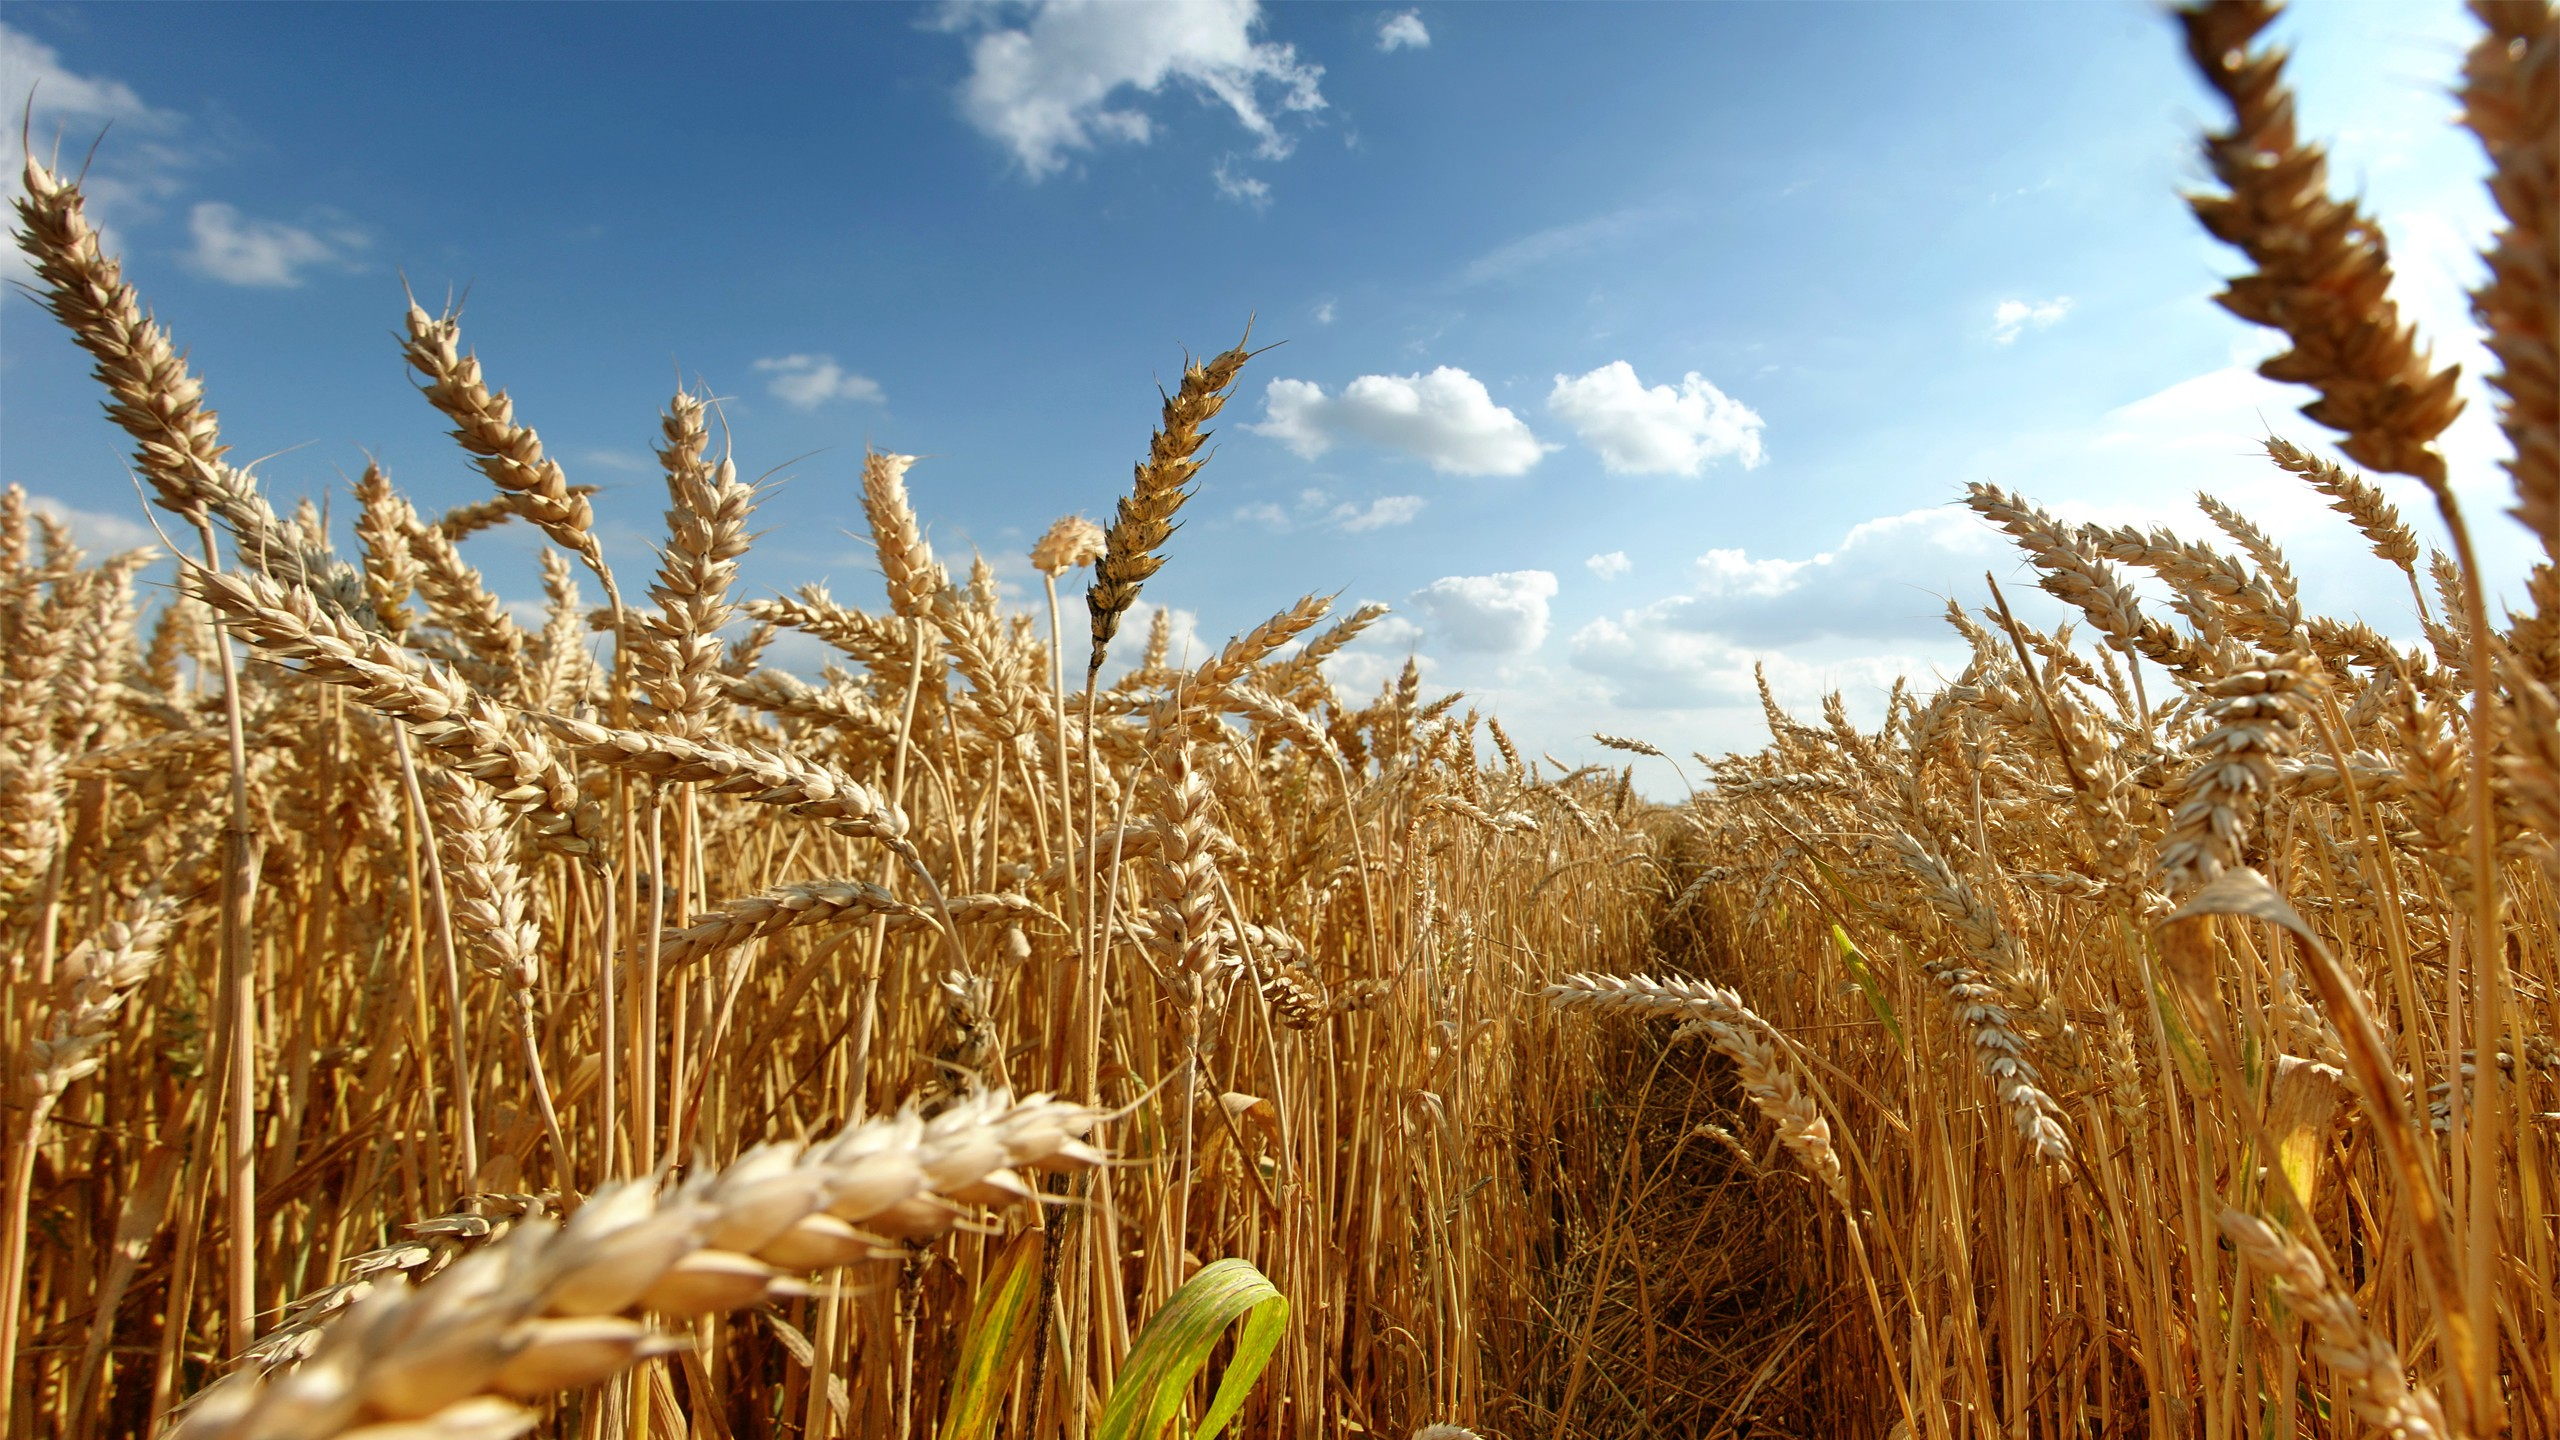
\includegraphics[width = 0.45\textwidth]{Wheat}
	\caption{Wheat \cite{Nature}.}
	
\end{wrapfigure}

This is some wheat. It's nice, isn't it? Remember that wrapfigure goes behind the text you want it to wrap in. For elegance, let's start a new paragraph properly.
\par
This time we will do 2 figures next to each other.\\\\
\\
\\


%Remember to add figure before dealing with subfigures
%You have to use [h] for pretty much every figure, this signifies "here" and tells latex to put the figure where you put it with respect to the order of the code

%Sometimes [h] doesn't really work, try removing the above \\ and the Meadow will overlap the "Figure 2.1 Wheat"
\begin{figure}[h]
	
	\begin{subfigure}{.5\textwidth}
		\centering
		%In subfigures, the width setting of graphics is with respect to the width of the subfigure, on this case. the width of the picture with respect to the normal width is 0.5*0.9
		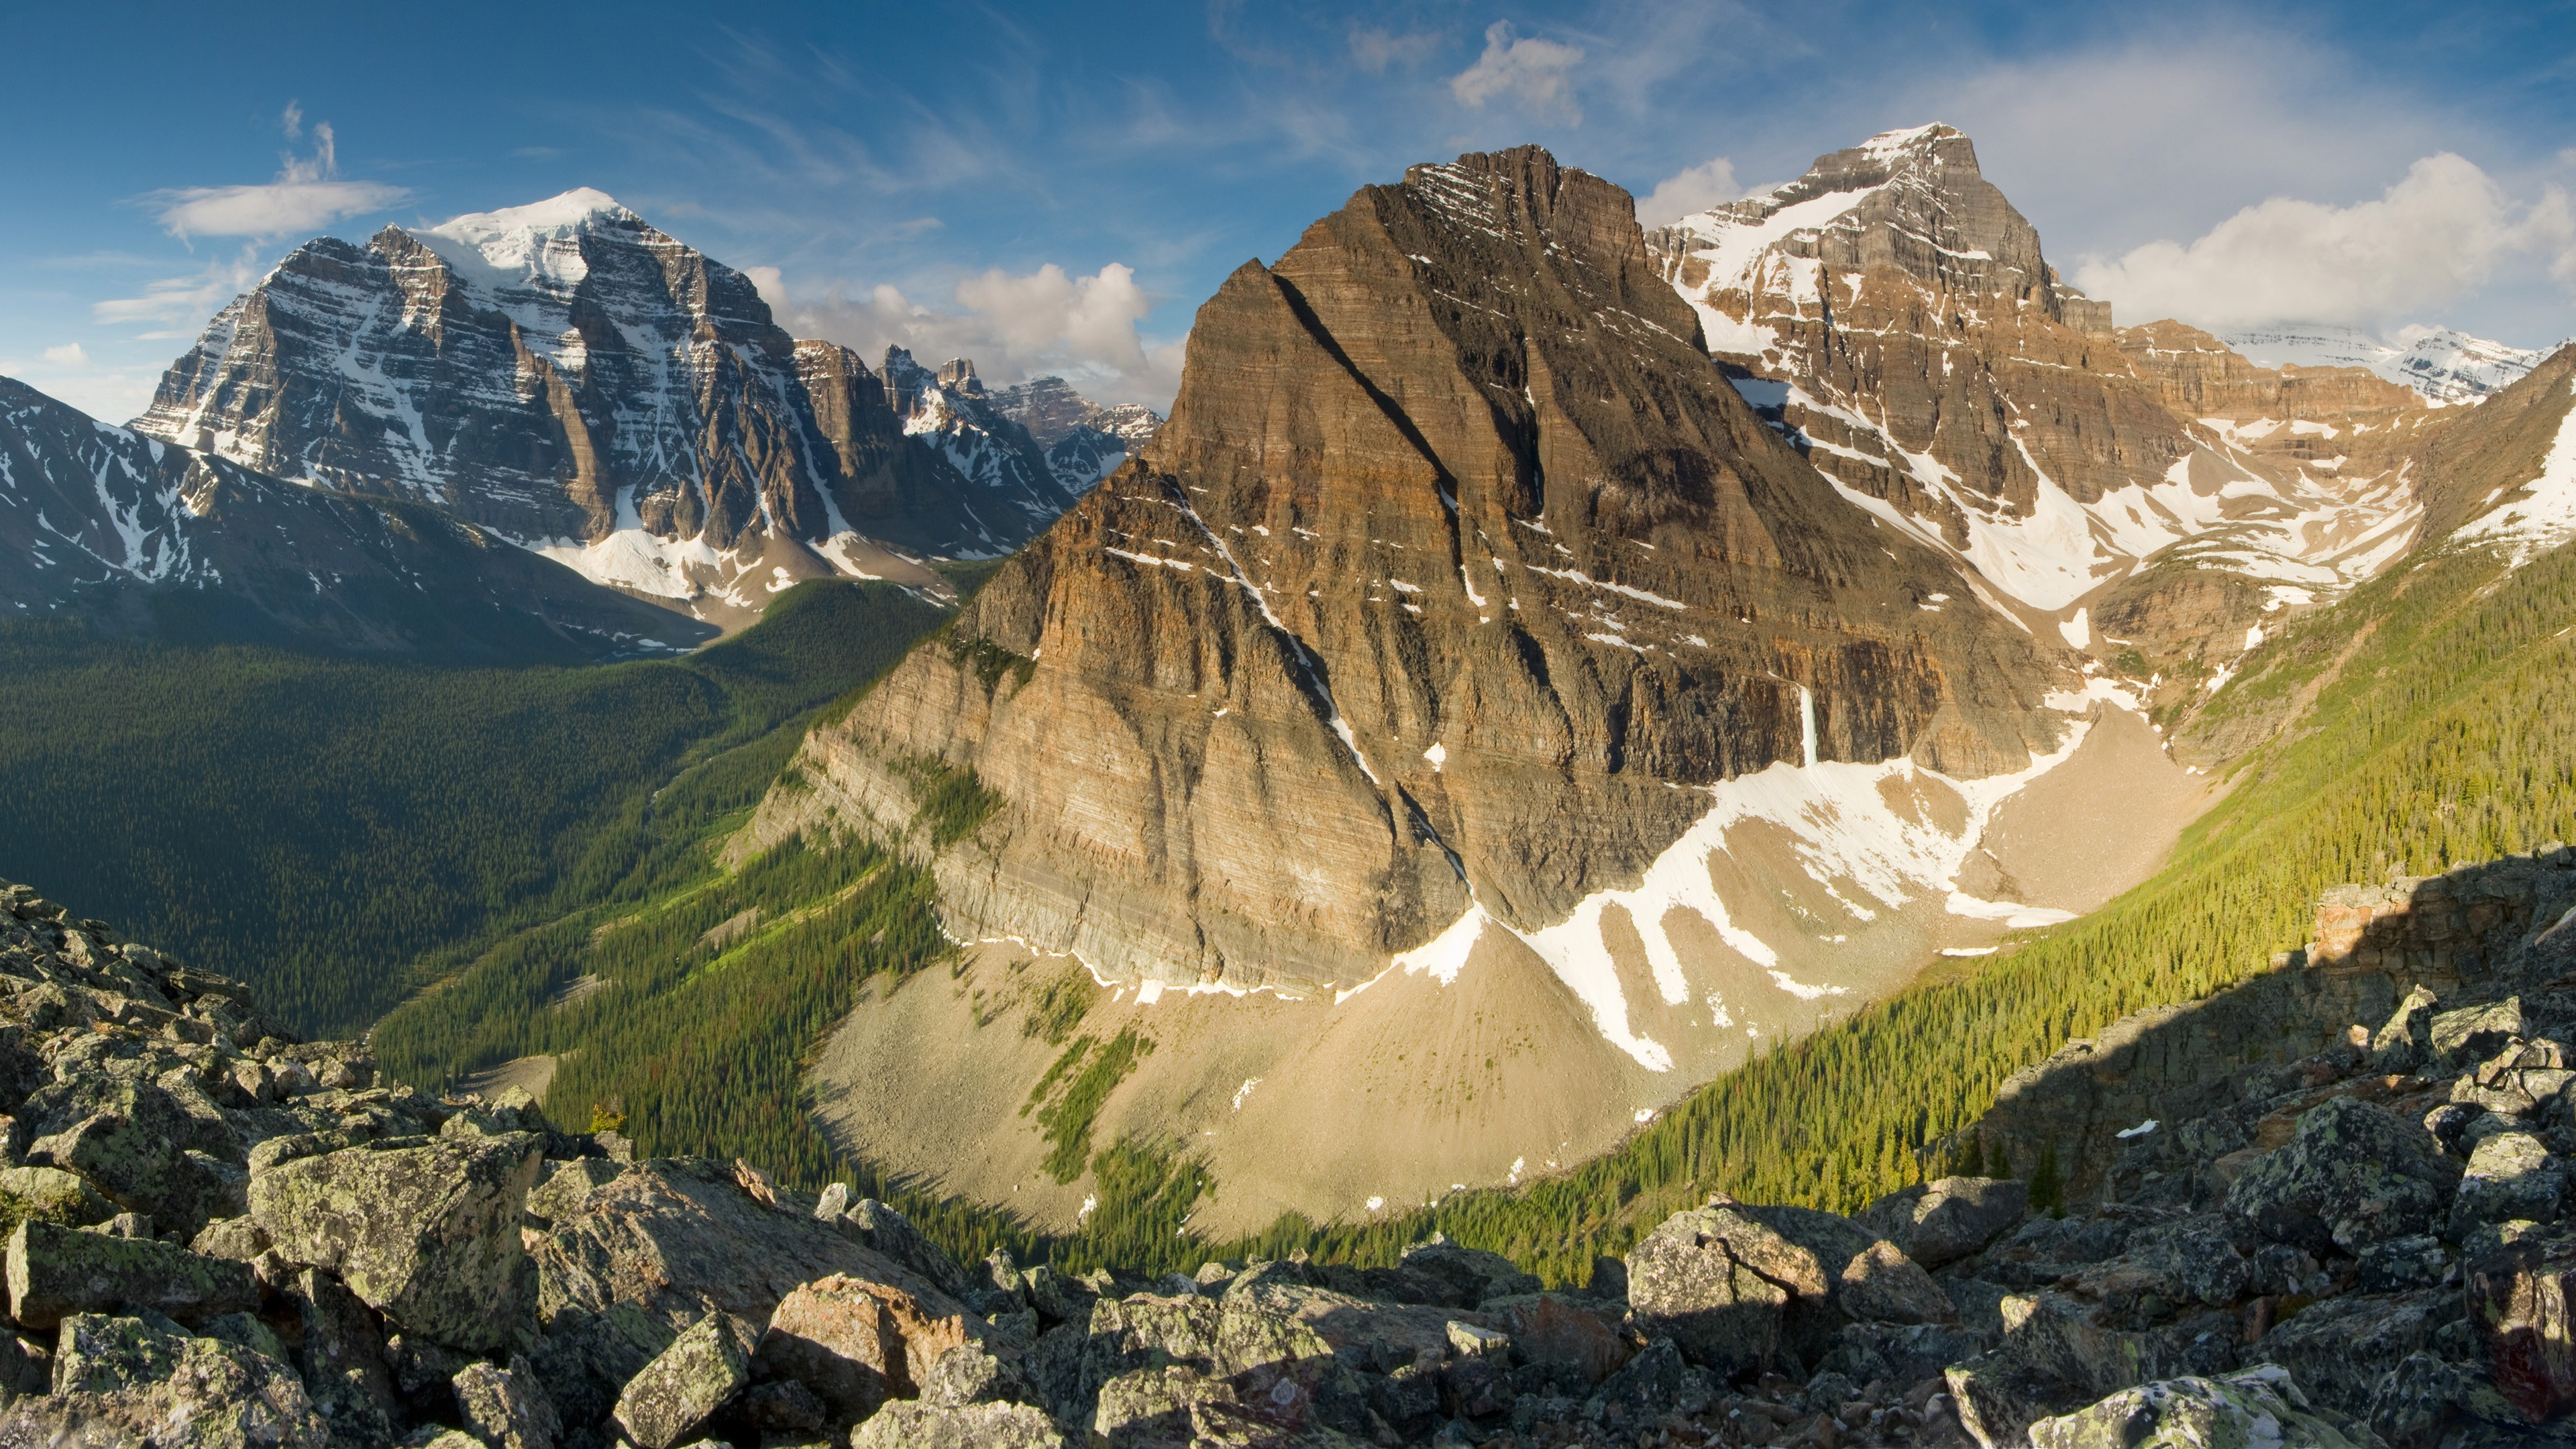
\includegraphics[width = 0.9\textwidth]{Mountains}
		\caption{Mountains \cite{Nature}.}
	%The percentage mark is crucial as it allows the two figures to be side by side
	\end{subfigure}%
	\begin{subfigure}{.5\textwidth}
		\centering
		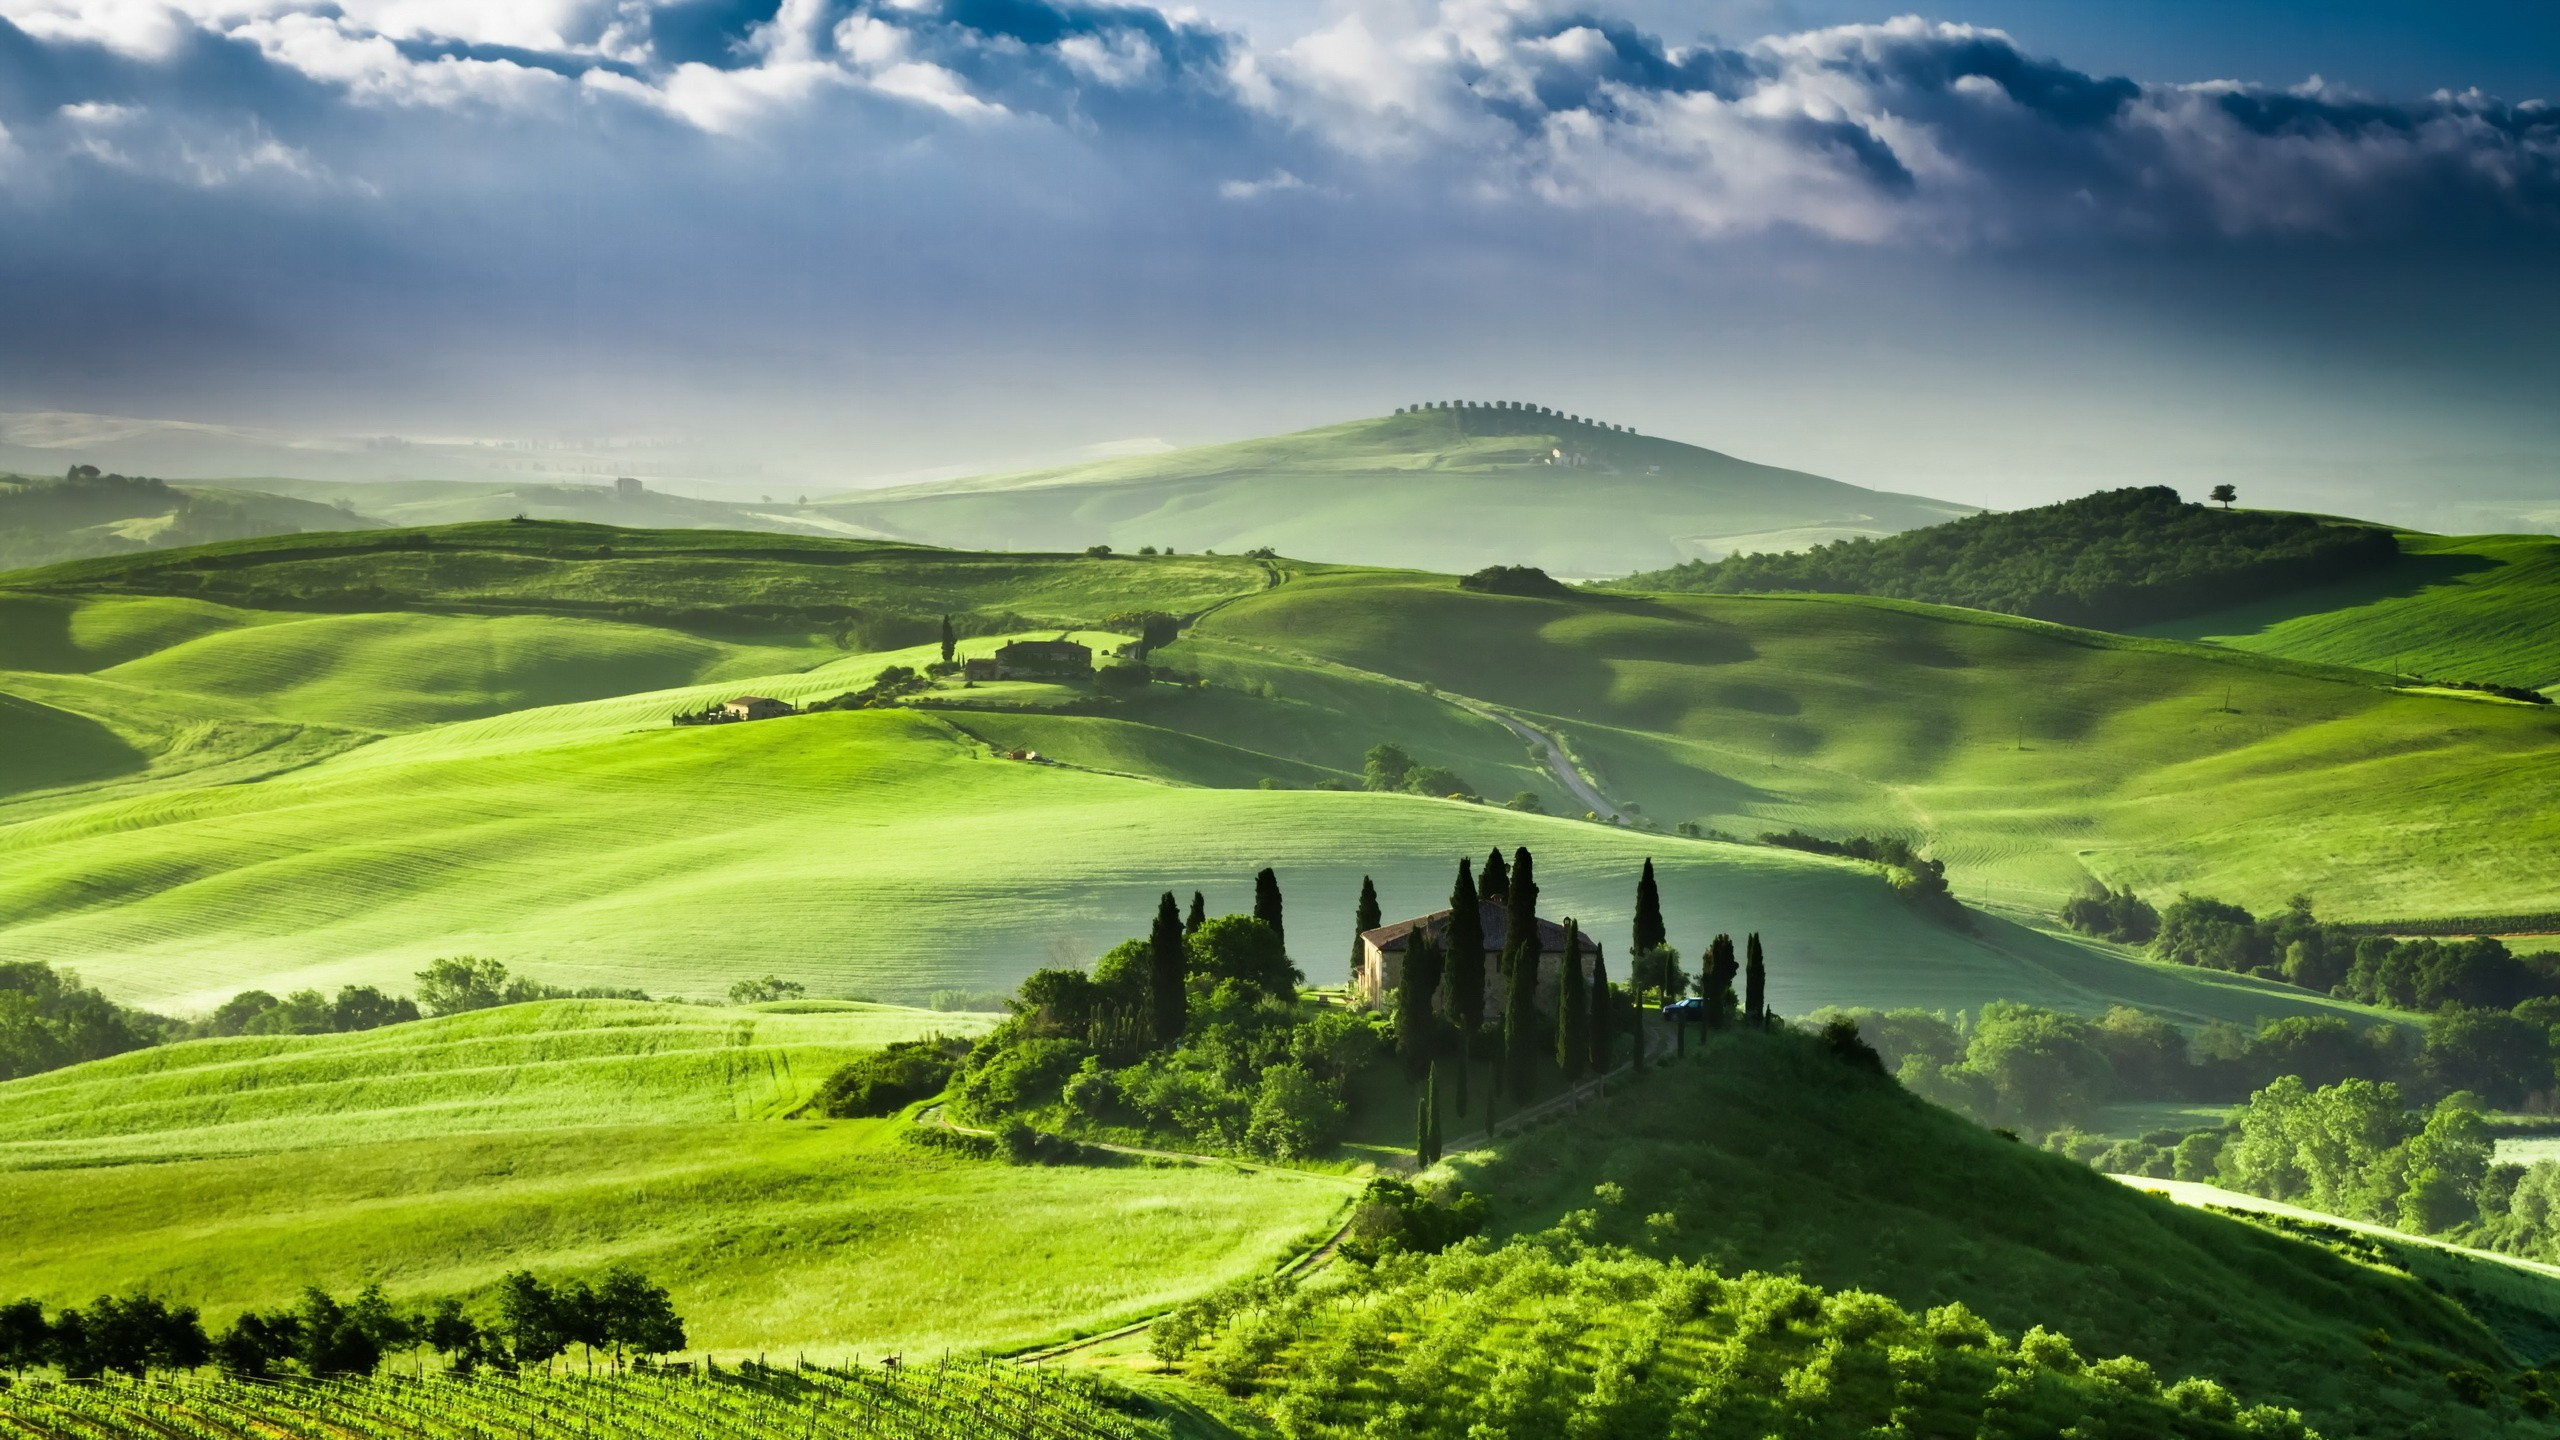
\includegraphics[width = 0.9\textwidth]{Meadow}
		\caption{Meadow \cite{Nature}.}
	\end{subfigure}
	\caption{Two figures}
	
\end{figure}

{For some reason, text alignment breaks here. However it's solved with brackets. I suppose they should be used whenever alignment problems arises.\\}

\newpage
\section*{Hidden Section... Shhhh}

%Number of multicolumns
\begin{multicols}{2}
	[We will start a multicolumn section. 
	Add square brackets to indicate that the text will span all the columns / be normal]
	
	The text in the two columns are automatically adjusted so that the height of them are equivalent. This makes it better than subfigures in certain circumstances .This doesn't really work if there's too little words. Wrapfigures works within these columns and again they will be automated.\\
\end{multicols}

\newpage

%Remember to start a bib file called References.bib before doing this step
%This generates the refernces page
\bibliography{References}

\end{document}